\begin{figure}[htbp]\centering
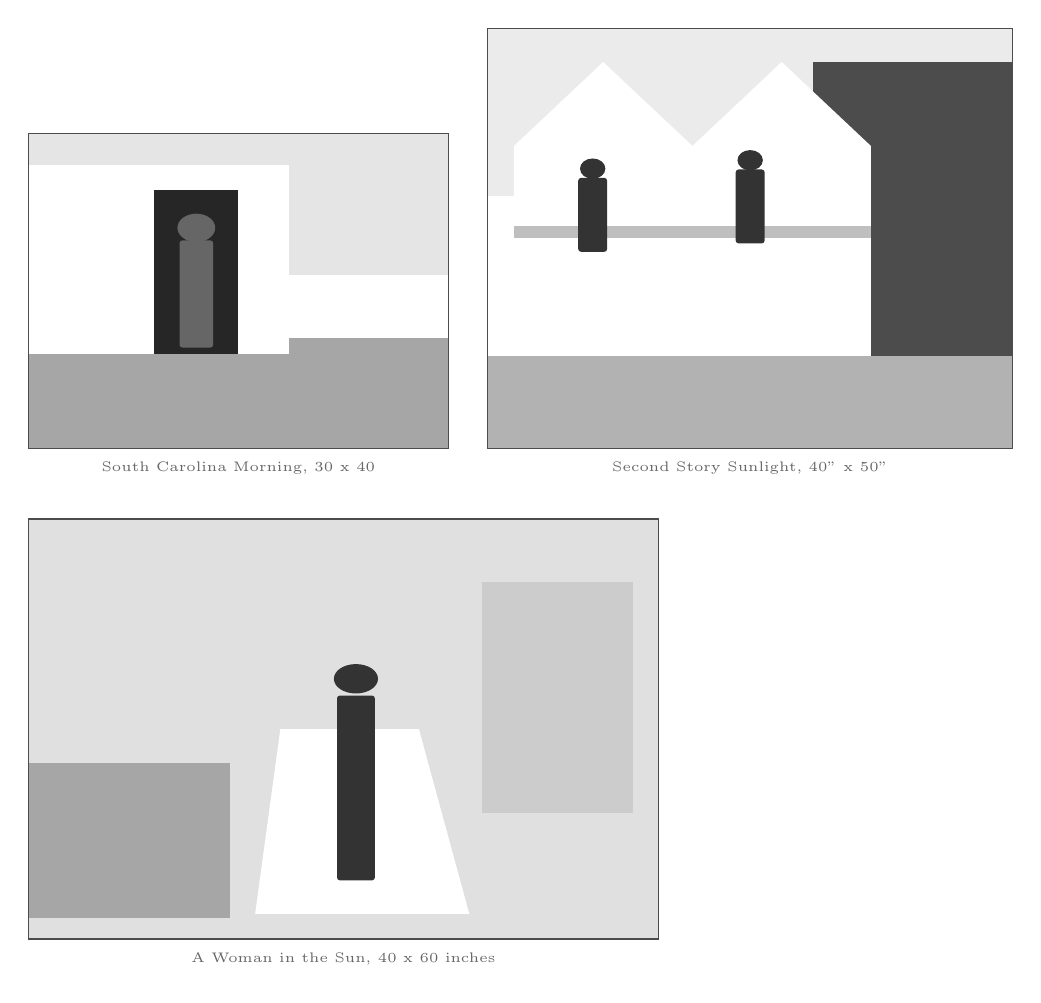
\begin{tikzpicture}
\begin{scope}[shift={(0,0)},x=5.333cm,y=4.000cm]\clip (0,0) rectangle (1,1);
\fill[black!10] (0,0.55) rectangle (1,1);           % sky
\fill[black!35] (0,0) rectangle (1,0.35);           % field
\fill[white] (0,0.3) rectangle (0.62,0.9);          % the house front
\fill[black!85] (0.3,0.3) rectangle (0.5,0.82);     % the doorway
\fill[black!60] (0.4,0.7) circle (0.045); \fill[black!60,rounded corners=1pt] (0.36,0.32) rectangle (0.44,0.66); % « Dinah »
\end{scope}
\draw[black!70,line width=0.5pt] (0,0) rectangle (5.333333333333333,4);
\node[anchor=north,font=\tiny,text=black!60] at (2.6666666666666665,-0.05) {South Carolina Morning, 30 x 40};
\begin{scope}[shift={(5.833333333333333,0)},x=6.667cm,y=5.333cm]\clip (0,0) rectangle (1,1);
\fill[black!8] (0,0.6) rectangle (1,1);             % sky
\fill[black!70] (0.62,0.2) rectangle (1,0.92);      % the woods behind
\fill[black!30] (0,0) rectangle (1,0.22);           % grass
\fill[white] (0.05,0.22) -- (0.05,0.72) -- (0.22,0.92) -- (0.39,0.72) -- (0.39,0.72) -- (0.56,0.92) -- (0.73,0.72) -- (0.73,0.22) -- cycle; % two gables
\fill[black!25] (0.05,0.5) rectangle (0.73,0.53);   % the balcony rail
\fill[black!80] (0.2,0.6659999999999999) circle (0.0242); \fill[black!80,rounded corners=1pt] (0.17250000000000001,0.46799999999999997) rectangle (0.2275,0.644); \fill[black!80] (0.5,0.6859999999999999) circle (0.0242); \fill[black!80,rounded corners=1pt] (0.4725,0.488) rectangle (0.5275,0.664);       % « Gothic + Elderly », « Toots »
\end{scope}
\draw[black!70,line width=0.5pt] (5.833333333333333,0) rectangle (12.5,5.333333333333333);
\node[anchor=north,font=\tiny,text=black!60] at (9.166666666666666,-0.05) {Second Story Sunlight, 40" x 50"};
\begin{scope}[shift={(0,-6.233333333333333)},x=8.000cm,y=5.333cm]\clip (0,0) rectangle (1,1);
\fill[black!12] (0,0) rectangle (1,1);
\fill[black!35] (0,0.05) rectangle (0.32,0.42);     % the bed
\fill[black!20] (0.72,0.3) rectangle (0.96,0.85);   % the window, landscape out of it
\fill[white] (0.36,0.06) -- (0.7,0.06) -- (0.62,0.5) -- (0.4,0.5) -- cycle; % « this Early light » on the floor
\fill[black!80] (0.52,0.62) circle (0.035); \fill[black!80,rounded corners=1pt] (0.49,0.14) rectangle (0.55,0.58); % the figure standing in it
\end{scope}
\draw[black!70,line width=0.5pt] (0,-6.233333333333333) rectangle (8,-0.9000000000000004);
\node[anchor=north,font=\tiny,text=black!60] at (4,-6.283333333333333) {A Woman in the Sun, 40 x 60 inches};
\end{tikzpicture}
\caption{\textbf{South Carolina Morning}, oil, 1955; « Dinah », 30 x 40 as the leaf writes it (Book III, leaf 53, ref 18558). Whitney Museum of American Art, 67.13: \url{https://whitney.org/collection/works/789}. \textbf{Second Story Sunlight}, oil, 25 August to 15 September 1960; « Toots », 40" x 50" as the leaf writes it (Book III, leaf 73, ref 17872). Whitney Museum of American Art, 60.54: \url{https://whitney.org/collection/works/873}. \textbf{A Woman in the Sun}, oil, October 1961; « the WISE TRAMP », 40 x 60 inches as the leaf writes it (Book III, leaf 75, ref 17107). Whitney Museum of American Art, 84.31: \url{https://whitney.org/collection/works/1337}. Scale: sixty inches to eight centimetres; the three formats of the last decade, 30 by 40, 40 by 50 and 40 by 60. The drawings are schemas of the composition in its main masses only, at the proportions of the size in Edward Hopper's hand, made from the leaf's description and from general knowledge of the picture; nothing is traced and no detail is drawn, and they are not reproductions. The pictures themselves are at the museums' own pages. Drawn by Claude Fable~5.1, 13 September 2026, from the transcriptions and \texttt{works.json} (2026-09-14).}\label{fig:late}
\end{figure}
